\documentclass[11pt]{article}

% ---------------- Packages ----------------
\usepackage[margin=1in]{geometry}
\usepackage{amsmath,amssymb,amsthm}
\usepackage{graphicx}
\usepackage{hyperref}
\usepackage{fancyhdr}
\usepackage{enumitem}
\usepackage[UTF8]{ctex}
\usepackage{algorithm}
\usepackage{algpseudocode}
% ---------------- Header ----------------
\pagestyle{fancy}
\fancyhf{}
\lhead{Course Name}
\rhead{Homework \#1}
\cfoot{\thepage}

% ---------------- Title ----------------
\title{Homework 1}
\author{羊瑞 \\ 2300013091}
\date{\today}

% ---------------- Custom commands ----------------
\newcommand{\R}{\mathbb{R}}
\newcommand{\E}{\mathbb{E}}

% ---------------- Problem Environment ----------------
\newcounter{problem}

\newenvironment{problem}[1][]{
\stepcounter{problem}
\section*{Problem \theproblem\; #1}
}{}

\newenvironment{solution}{
\par\noindent\textbf{Solution.}\par\noindent
}{\qed}

\setlength{\parindent}{0pt}
% ---------------- Document ----------------
\begin{document}

\maketitle

\begin{problem} 
\begin{center}
    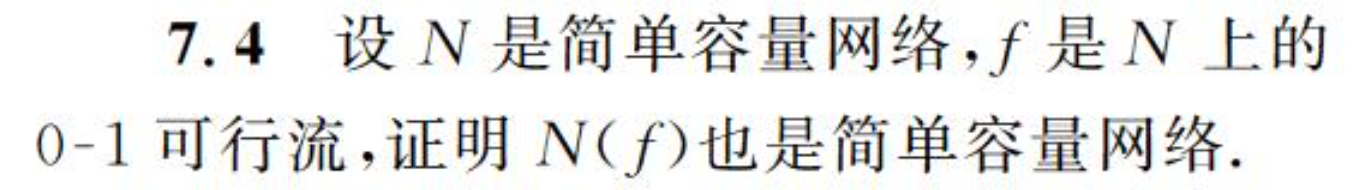
\includegraphics[width=0.6\textwidth]{problems/7-4.png}
\end{center}
\end{problem}

\begin{solution}
证明:
因为 \(N\) 是简单容量网络，所以对任意两点 \(i,j\in V\)，若
$(i,j) \in E$, 则
$(j,i)\notin E.$
并且简单容量网络中每条弧的容量为 \(1\)，即
$
c(i,j)=1,\qquad \forall (i,j)\in E.
$

又因为 \(f\) 是 \(0\)-\(1\) 可行流，所以对任意 \((i,j)\in E\)，有
$
f(i,j)\in \{0,1\}.
$ 

由 \(f\) 构造的辅助网络 \(N(f)\) 的弧集记为 \(E(f)\)。对原网络中的任意一条弧 \((i,j)\in E\)，有两种情况：

$
\begin{cases}
f(i,j)=0, & \text{则在 }N(f)\text{ 中保留正向弧 }(i,j), \\
f(i,j)=1, & \text{则在 }N(f)\text{ 中加入反向弧 }(j,i).
\end{cases}
$

因此
$
E(f)
=
\{(i,j)\mid (i,j)\in E,\ f(i,j)=0\}
\cup
\{(j,i)\mid (i,j)\in E,\ f(i,j)=1\}.
$

假设存在两个顶点 \(i,j\in V\)，使得
$
(i,j)\in E(f)
\quad\text{且}\quad
(j,i)\in E(f).
$

由于 \(N\) 是简单容量网络，在原网络 \(N\) 中不可能同时存在
$
(i,j)\in E
\quad\text{和}\quad
(j,i)\in E.
$

若原网络中存在的是 \((i,j)\in E\)，则因为
$
f(i,j)\in\{0,1\},
$
只有两种情况：

$
f(i,j)=0
\quad\Rightarrow\quad
(i,j)\in E(f),\ (j,i)\notin E(f),
$

$
f(i,j)=1
\quad\Rightarrow\quad
(j,i)\in E(f),\ (i,j)\notin E(f).
$

因此不可能同时有
$
(i,j)\in E(f)
\quad\text{和}\quad
(j,i)\in E(f).
$

同理，若原网络中存在的是 \((j,i)\in E\)，也不可能在 \(N(f)\) 中同时出现 \((i,j)\) 和 \((j,i)\)。

这与假设矛盾。因此，\(N(f)\) 中任意两点之间也不可能同时存在反向弧。

再看容量。若 \((i,j)\in E\) 且 \(f(i,j)=0\)，则 \(N(f)\) 中正向弧 \((i,j)\) 的剩余容量为
$
c(i,j)-f(i,j)=1-0=1.
$
若 \((i,j)\in E\) 且 \(f(i,j)=1\)，则 \(N(f)\) 中反向弧 \((j,i)\) 的容量为
$
f(i,j)=1.
$

所以 \(N(f)\) 中每条弧的容量仍然为 \(1\)。

综上，\(N(f)\) 满足：
\text{每条弧的容量为 }1,
\text{任意两点之间不同时存在反向弧}.

因此，\(N(f)\) 也是简单容量网络。

\end{solution}

\begin{problem}
\begin{center}
    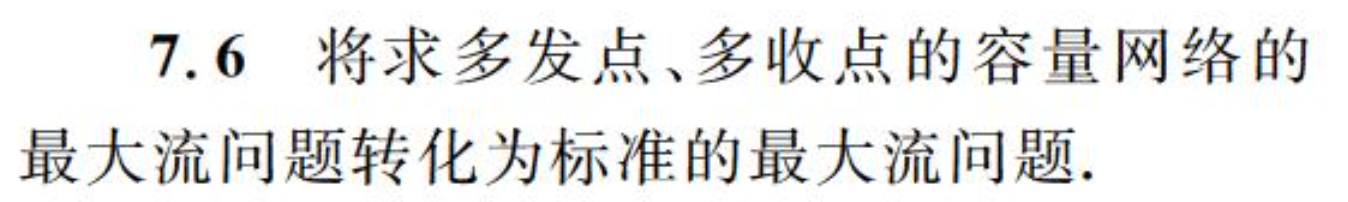
\includegraphics[width=0.6\textwidth]{problems/7-6.png}
\end{center}
\end{problem}

\begin{solution}
设多发点集合为
$
S=\{s_1,s_2,\dots,s_k\},
$
多收点集合为
$
T=\{t_1,t_2,\dots,t_m\}.
$

构造新网络
$
N'=(V',E',c',s_0,t_0),
$
其中
$
V'=V\cup\{s_0,t_0\},
$
$
E'=E\cup\{(s_0,s_i)\mid s_i\in S\}
\cup\{(t_j,t_0)\mid t_j\in T\}.
$

对原有弧 \((u,v)\in E\)，令
$
c'(u,v)=c(u,v).
$

对新增弧，令
$
c'(s_0,s_i)=+\infty,\qquad i=1,2,\dots,k,
$
$
c'(t_j,t_0)=+\infty,\qquad j=1,2,\dots,m.
$

若各发点有供给上限 \(b_i\)，则令
$
c'(s_0,s_i)=b_i.
$

若各收点有需求或接收上限 \(d_j\)，则令
$
c'(t_j,t_0)=d_j.
$

于是 \(N'\) 是只有一个源点 \(s_0\) 和一个汇点 \(t_0\) 的标准容量网络。原多发点、多收点网络的最大流值等于新网络 \(N'\) 中从 \(s_0\) 到 \(t_0\) 的最大流值。
\end{solution}

\begin{problem}
\begin{center}
    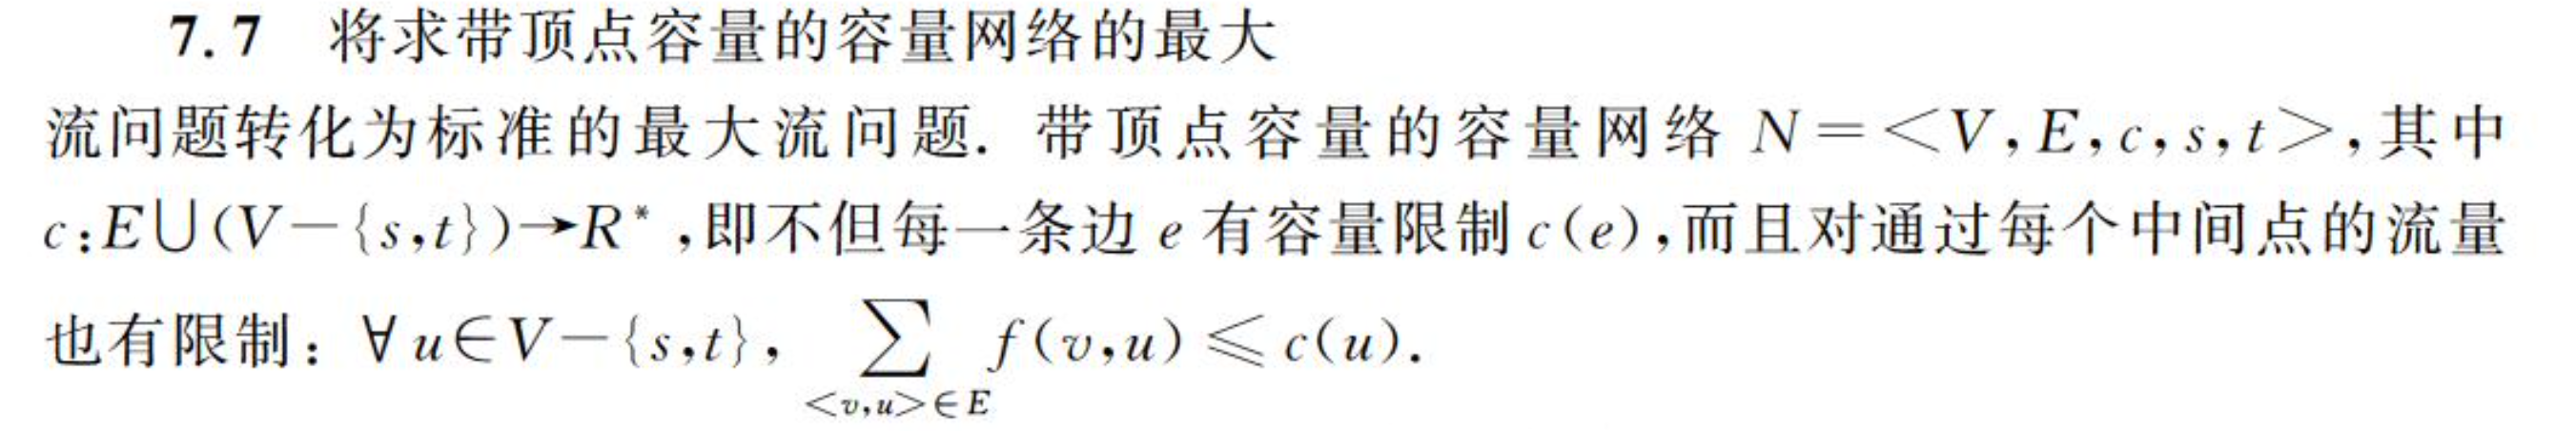
\includegraphics[width=0.6\textwidth]{problems/7-7.png}
\end{center}
\end{problem}

\begin{solution}
设原网络为
$
N=(V,E,c,s,t),
$
其中每条边 \((u,v)\in E\) 有边容量 \(c(u,v)\)，并且每个中间点
$
u\in V-\{s,t\}
$
有点容量 \(c(u)\)。

构造一个标准容量网络
$
N'=(V',E',c',s,t).
$

对每个中间点 \(u\in V-\{s,t\}\)，将其拆成两个点
$
u^-,\quad u^+,
$
并加入一条边
$
(u^-,u^+),
$
其容量定义为
$
c'(u^-,u^+)=c(u).
$

源点 \(s\) 和汇点 \(t\) 不拆分。因此新点集为
$
V'=\{s,t\}\cup \{u^-,u^+\mid u\in V-\{s,t\}\}.
$

对原网络中的每条边 \((u,v)\in E\)，在新网络中加入一条对应边
$
(\operatorname{out}(u),\operatorname{in}(v)),
$
其中
$
\operatorname{out}(u)=
\begin{cases}
s, & u=s,\\
u^+, & u\in V-\{s,t\},\\
t, & u=t,
\end{cases}
$
$
\operatorname{in}(v)=
\begin{cases}
s, & v=s,\\
v^-, & v\in V-\{s,t\},\\
t, & v=t.
\end{cases}
$

并令其容量为
$
c'(\operatorname{out}(u),\operatorname{in}(v))=c(u,v).
$

于是
$
E'
=
\{(u^-,u^+)\mid u\in V-\{s,t\}\}
\cup
\{(\operatorname{out}(u),\operatorname{in}(v))\mid (u,v)\in E\}.
$

下面说明该构造的正确性。

在新网络中，任意通过中间点 \(u\) 的流都必须经过边
$
u^- \to u^+.
$
而该边的容量为
$
c'(u^-,u^+)=c(u).
$
因此流过原点 \(u\) 的总流量不会超过 \(c(u)\)。

同时，原网络中的每条边 \((u,v)\) 都对应新网络中的一条边
$
(\operatorname{out}(u),\operatorname{in}(v)),
$
且容量保持不变，因此原来的边容量限制也被保留。

所以，原带点容量网络 \(N\) 中的任意可行流都可以对应为新网络 \(N'\) 中的一个可行流；反过来，\(N'\) 中的任意可行流也可以还原为 \(N\) 中满足点容量限制的可行流。

因此，带点容量的最大流问题可以转化为标准最大流问题，且二者最大流值相等。
\end{solution}

\begin{problem}
\begin{center}
    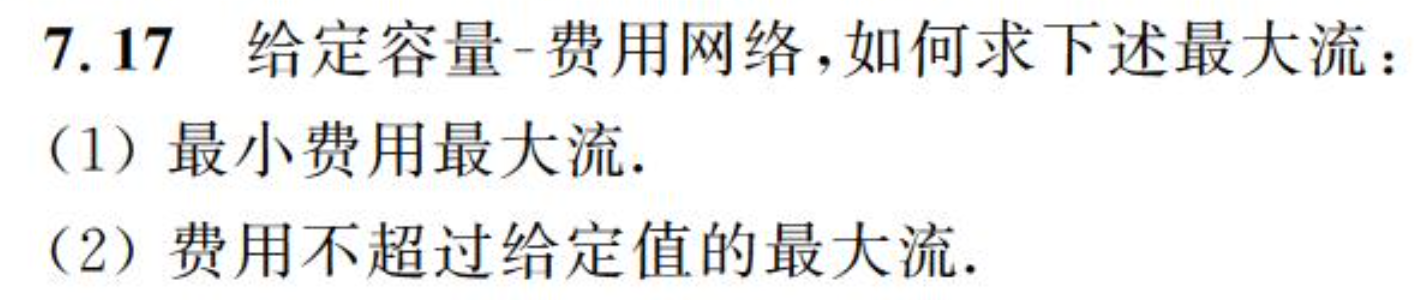
\includegraphics[width=0.6\textwidth]{problems/7-17.png}
\end{center}
\end{problem}

\begin{solution}
(1) \\
1. 调用最大流算法求出最大流f. \\
2. 构造N(f). \\
3. 调用Floyd算法检测N(f)中是否有权aw的负回路C，若存在，goto 4；否则输出f，结束. \\
4. 令 $d = min \{ac(i, j) | <i, j> \in E(C)\} $ \\
5. 对 $<i, j> \in E(C), 若<i, j> \in E, f(i, j)+=d; 若<j, i> \in E, f(i, j)-=d. $ \\
6. goto 2. \\
\\
(2) \\
1. 调用最大流算法求出最大流f. \\
2. 构造N(f). \\
3. 设给定费用w, 当w(f)<=w时，结束。若N(f)中有权aw的负回路C, goto 4; 若不然， 无解. \\
4. 令$d = min \{ac(i, j) | <i, j> \in E(C)\} $ \\
5. 对 $<i, j> \in E(C), 若<i, j> \in E, f(i, j)+=d; 若<j, i> \in E, f(i, j)-=d. $ \\
6. goto 3. \\
\end{solution}

\begin{problem}
\begin{center}
    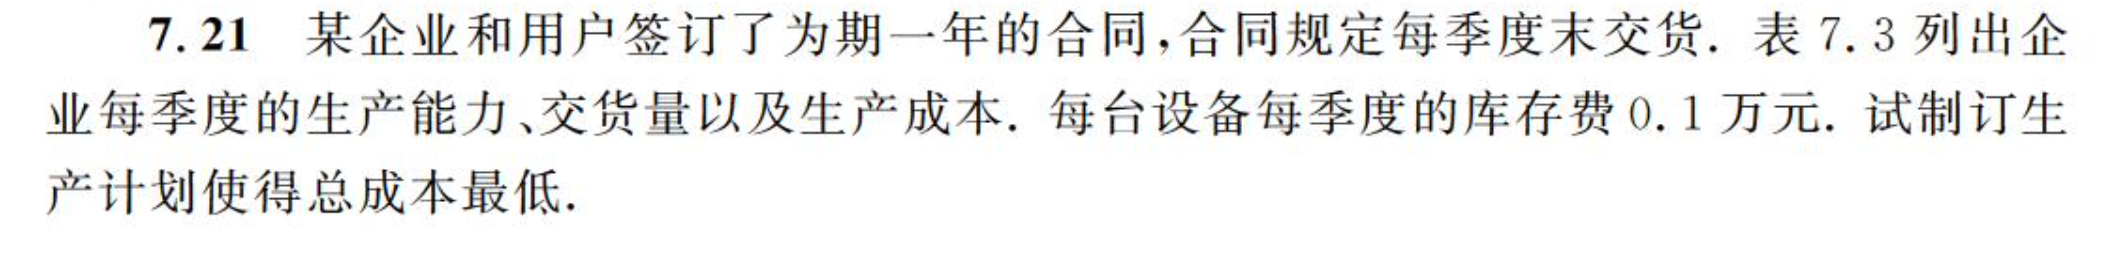
\includegraphics[width=0.6\textwidth]{problems/7-21.1.png}
    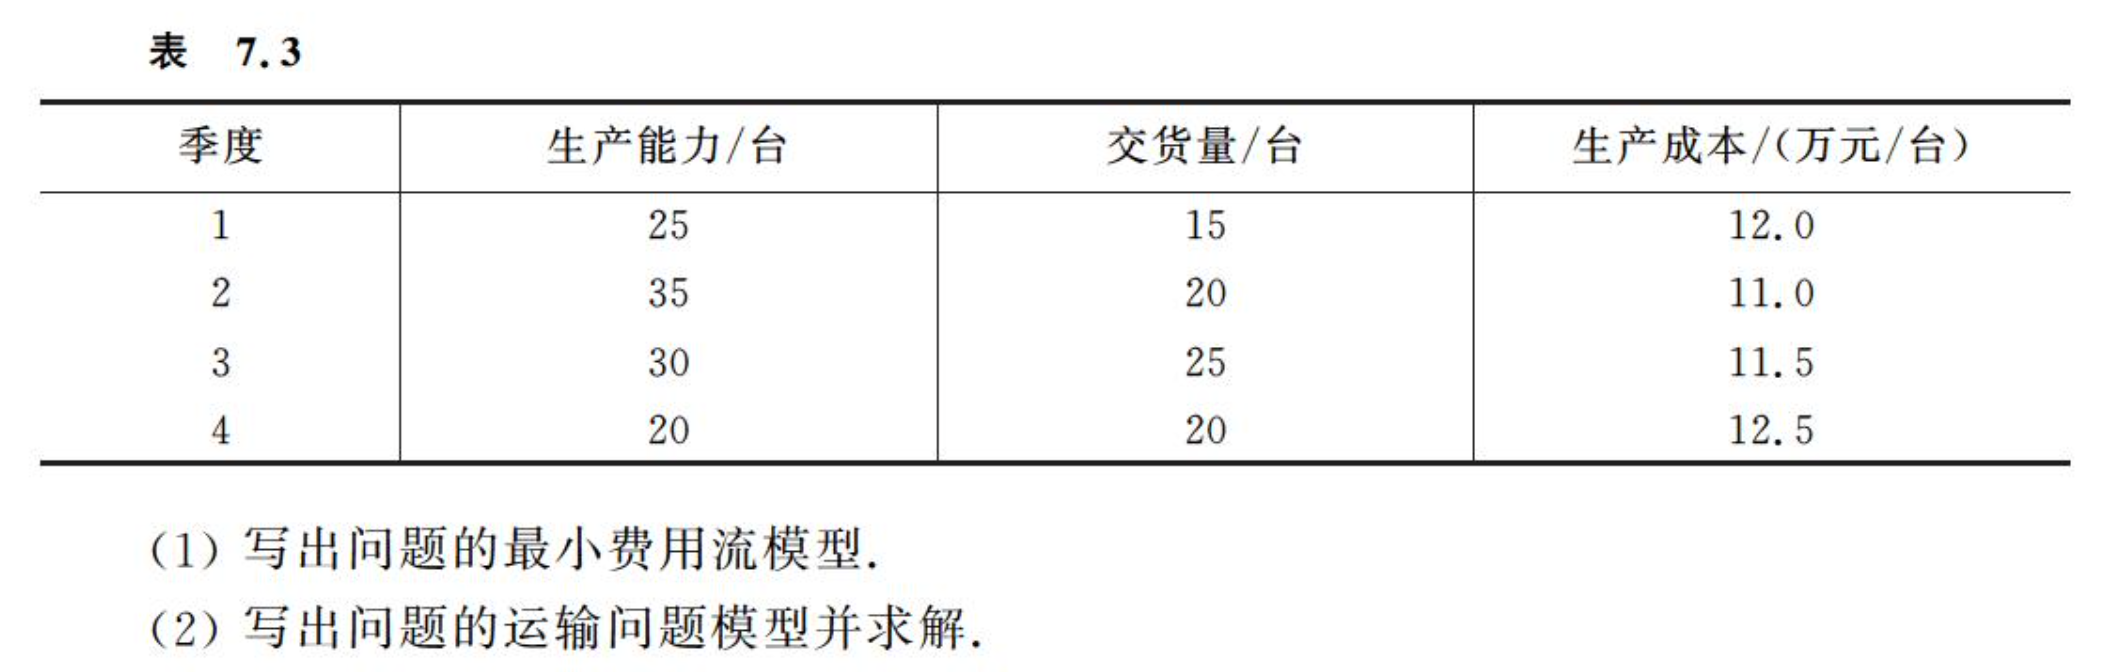
\includegraphics[width=0.6\textwidth]{problems/7-21.2.png}
\end{center}
\end{problem}

\begin{solution}
(1)
设四个季度对应节点为
$
1,2,3,4.
$
增加源点 \(s\) 和汇点 \(t\)，构造容量--费用网络
$
N=(V,E,c,w,s,t).
$

其中
$
V=\{s,1,2,3,4,t\}.
$

从源点到各季度节点连边
$
(s,i),\quad i=1,2,3,4,
$
表示第 \(i\) 季度的生产。其容量和费用分别为
$
c(s,1)=25,\quad w(s,1)=12.0,
$
$
c(s,2)=35,\quad w(s,2)=11.0,
$
$
c(s,3)=30,\quad w(s,3)=11.5,
$
$
c(s,4)=20,\quad w(s,4)=12.5.
$

从各季度节点到汇点连边
$
(i,t),\quad i=1,2,3,4,
$
表示第 \(i\) 季度交货。其容量为对应季度交货量，费用为 \(0\)，即
$
c(1,t)=15,\quad w(1,t)=0,
$
$
c(2,t)=20,\quad w(2,t)=0,
$
$
c(3,t)=25,\quad w(3,t)=0,
$
$
c(4,t)=20,\quad w(4,t)=0.
$

再加入库存边
$
(1,2),(2,3),(3,4),
$
表示将本季度生产的设备库存到下一季度。其容量设为充分大，费用为库存费：
$
c(1,2)=c(2,3)=c(3,4)=+\infty,
$
$
w(1,2)=w(2,3)=w(3,4)=0.1.
$

总交货量为
$
15+20+25+20=80.
$
因此，原问题可转化为在该容量--费用网络中求流量值为
$
v=80
$
的最小费用流问题，即
$
\min \sum_{(i,j)\in E} w(i,j)f(i,j),
$
满足
$
0\leq f(i,j)\leq c(i,j),\qquad \forall (i,j)\in E,
$
以及除 \(s,t\) 外各节点的流量守恒条件，并且
$
|f|=80.
$
\end{solution}


\end{document}